%----------------------------------------------------------------------------------------
%	CARDIO-CODE presentation, Team Ramanujan, Milan 2K26
%	Style taken from the team's Beamer template (Madrid + orchid). Compile from this folder:
%	    pdflatex cardio_code_slides.tex      (or: tectonic cardio_code_slides.tex)
%	Figures are read from ../plots/
%----------------------------------------------------------------------------------------
\documentclass[t,aspectratio=169]{beamer}

\newcommand*\lev{\item[\color{red}\scalebox{0.9}{\textbullet}]}
\usepackage[font=scriptsize,labelfont=bf]{caption}

\mode<presentation>{
  \usetheme{Madrid}
  \usecolortheme{orchid}
  \setbeamertemplate{navigation symbols}{}
}

\usepackage{graphicx}
\usepackage{booktabs}
\usepackage{amsmath}
\usepackage{amssymb}
\usepackage{tikz}
\usetikzlibrary{positioning,arrows.meta}
\usefonttheme{professionalfonts}
\graphicspath{{../plots/}}
\newcommand{\code}[1]{\texttt{#1}}
\newcommand{\plain}[1]{{\color{gray}\textit{(#1)}}}

\setbeamertemplate{footline}{%
  \leavevmode%
  \hbox{\begin{beamercolorbox}[wd=.5\paperwidth,ht=2.5ex,dp=1.125ex,leftskip=.3cm plus1fill,rightskip=.3cm]{author in head/foot}%
    \usebeamerfont{author in head/foot}\insertshorttitle
  \end{beamercolorbox}%
  \begin{beamercolorbox}[wd=.5\paperwidth,ht=2.5ex,dp=1.125ex,leftskip=.3cm,rightskip=.3cm plus1fil]{title in head/foot}%
    \usebeamerfont{title in head/foot}Team Ramanujan \hspace{5mm} Milan 2K26 \hspace{13mm}\insertframenumber{}/\inserttotalframenumber
  \end{beamercolorbox}}%
}

%----------------------------------------------------------------------------------------
%	TITLE PAGE
%----------------------------------------------------------------------------------------
\title[CARDIO-CODE]{CARDIO-CODE\\[1ex]\large DSP-Driven Arrhythmia Detection in Motion-Corrupted PPG}
\subtitle{Signal processing only, no machine learning}
\author[Team Ramanujan]{Darshan, Piyush\\[0.5ex]\textbf{Team Ramanujan}}
\institute[]{Milan 2K26}
\date{October 2026}

\begin{document}

\begin{frame}[plain]
\titlepage
\end{frame}

\begin{frame}
\frametitle{Overview}
\tableofcontents[hideallsubsections]
\end{frame}

%----------------------------------------------------------------------------------------
\section{Problem}
%----------------------------------------------------------------------------------------
\begin{frame}
\frametitle{The Problem}
\framesubtitle{A heartbeat hidden in noise}
\begin{columns}[T]
\column{0.55\textwidth}
\begin{block}{A wearable story}
\begin{itemize}
  \item A wrist band records a few seconds of irregular heartbeat during a walk.
  \item Arm swing adds pulse-like waves; sweat makes the signal drift.
  \item The irregular beats are hidden, and \textbf{nothing flags them}.
\end{itemize}
\end{block}
\begin{exampleblock}{Our goal}
The software layer between a noisy signal and a \textbf{trustworthy, flagged insight}.
\end{exampleblock}
\column{0.42\textwidth}
\begin{alertblock}{Why it is hard}
\begin{itemize}
  \lev Arm motion (about 1--2\,Hz) sits in the \textbf{same frequency range} as the pulse.
  \lev A fixed filter cannot separate them.
  \lev Irregular rhythm must not be mistaken for noise, and noise must not be mistaken for irregular rhythm.
\end{itemize}
\end{alertblock}
\end{columns}
\end{frame}

\begin{frame}
\frametitle{Task, Output and Constraints}
\begin{columns}[T]
\column{0.58\textwidth}
\begin{block}{Output: \code{predictions.csv}, one row per input sample}
\scriptsize
\begin{tabular}{@{}ll@{}}
\toprule
\code{Timestamp} & time of the sample (s)\\
\code{Is\_peak} & 1 if a heartbeat peak is here\\
\code{Ibi\_ms} & time between the last two beats (ms)\\
\code{ano\_flag} & 1 inside a suspected abnormal rhythm\\
\code{confidence\_score} & 0--1: how far this part can be trusted\\
\bottomrule
\end{tabular}
\end{block}
\begin{block}{Input}
\small CSV with a PPG \plain{optical pulse} or ECG \plain{electrical} column; optional time and accelerometer
columns.
\end{block}
\column{0.39\textwidth}
\begin{alertblock}{Constraints}
\small
\begin{itemize}
  \item Time-domain or short-time spectral processing only.
  \item No ML, neural networks or pretrained models.
  \item Every step explainable.
\end{itemize}
\end{alertblock}
\begin{exampleblock}{Scoring criteria}
\small
\begin{itemize}
  \item Signal accuracy
  \item Anomaly detection
  \item Computational efficiency
\end{itemize}
\end{exampleblock}
\end{columns}
\end{frame}

\begin{frame}
\frametitle{The Data We Were Given}
\begin{block}{\code{ecg.csv}: MIT-BIH record 231}
\begin{itemize}
  \item 650\,000 samples at 360\,Hz (30.1\,min), two ECG leads.
  \item Contains a \textbf{2:1 AV heart block}: every second beat is dropped.
  \begin{itemize}
    \lev Normal rhythm: IBI $\approx$ 961\,ms (62\,bpm).
    \lev Block: IBI $\approx$ 1657\,ms (36\,bpm).
  \end{itemize}
\end{itemize}
\end{block}
\begin{exampleblock}{Two consequences for our design}
\begin{enumerate}
  \item The anomaly is \textbf{slow and regular}, not AF, so we need several independent rules, not just one
        irregularity test.
  \item The hidden test is \textbf{motion-corrupted PPG}, but our data is clean ECG, so we built our own stress tests
        with known answers, and the program picks ECG or PPG processing automatically.
\end{enumerate}
\end{exampleblock}
\end{frame}

%----------------------------------------------------------------------------------------
\section{Our Pipeline}
%----------------------------------------------------------------------------------------
\begin{frame}
\frametitle{Pipeline Overview}
\vspace{4mm}
\begin{center}
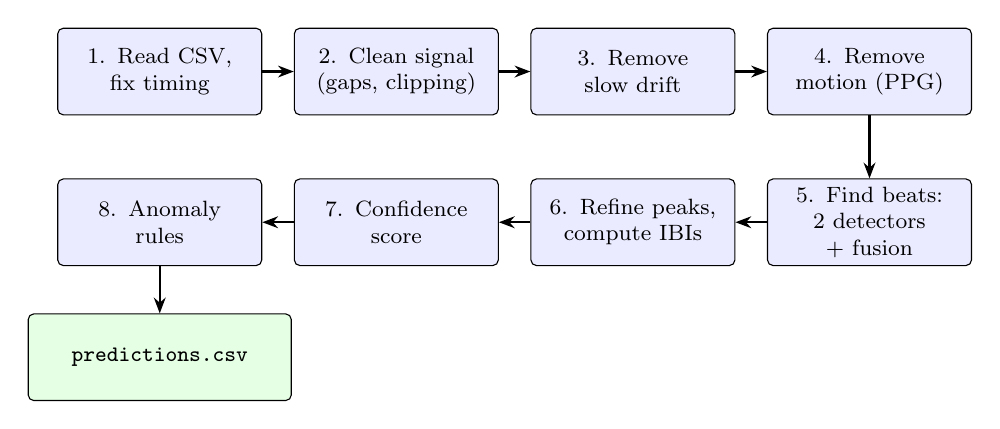
\begin{tikzpicture}[
  box/.style={draw,rounded corners=2pt,fill=blue!8,align=center,font=\footnotesize,
              minimum height=1.1cm,text width=2.45cm,inner sep=2pt},
  arr/.style={-{Stealth[length=2mm]},thick}, node distance=0.4cm]
\node[box] (a) {1. Read CSV,\\fix timing};
\node[box,right=of a] (b) {2. Clean signal\\(gaps, clipping)};
\node[box,right=of b] (c) {3. Remove\\slow drift};
\node[box,right=of c] (d) {4. Remove\\motion (PPG)};
\node[box,below=0.8cm of d] (e) {5. Find beats:\\2 detectors + fusion};
\node[box,left=of e] (f) {6. Refine peaks,\\compute IBIs};
\node[box,left=of f] (g) {7. Confidence\\score};
\node[box,left=of g] (h) {8. Anomaly\\rules};
\node[box,below=0.6cm of h,fill=green!10,text width=3.2cm] (i) {\code{predictions.csv}};
\draw[arr] (a)--(b); \draw[arr] (b)--(c); \draw[arr] (c)--(d); \draw[arr] (d)--(e);
\draw[arr] (e)--(f); \draw[arr] (f)--(g); \draw[arr] (g)--(h); \draw[arr] (h)--(i);
\end{tikzpicture}
\end{center}
\vspace{2mm}
\small ECG and PPG share this flow and differ in steps 3--5: an ECG beat is a sharp spike, a PPG beat is a smooth
hump. The mode is chosen from the column name, or from the frequency content.
\end{frame}

\begin{frame}
\frametitle{Steps 1--3: Input, Cleaning and Drift}
\begin{block}{Input handling}
\begin{itemize}
  \item The delimiter, column roles (by name) and time unit are detected automatically.
  \item Jittery or out-of-order timestamps are resampled onto an even grid.
  \item NaN runs and gaps longer than 1\,s are invalid: no beats, confidence 0.
\end{itemize}
\end{block}
\begin{block}{Baseline wander (slow drift)}
\begin{itemize}
  \item \textbf{Butterworth filter} \plain{a standard, smooth frequency sieve}, run \textbf{zero-phase}: forwards,
        then backwards, so beats do not shift in time.
  \item ECG: 0.5\,Hz high-pass. PPG: 0.5--8\,Hz band-pass.
  \item ECG only: adaptive 50/60\,Hz \textbf{notch} \plain{removes mains hum}, used only if the hum is
        $>$10\,dB above its surroundings.
\end{itemize}
\end{block}
\end{frame}

\begin{frame}
\frametitle{Step 4: Motion Artifact in PPG}
\framesubtitle{Two paths}
\small
\begin{columns}[T]
\column{0.48\textwidth}
\begin{block}{With accelerometer columns}
\textbf{NLMS adaptive filter} \plain{keeps re-tuning itself to predict how arm motion leaks into the PPG, then
subtracts it}
\begin{itemize}
  \lev 8 taps per axis, step size 0.01, runs at about 25\,Hz.
  \lev Used only if PPG/accelerometer \textbf{coherence} \plain{how strongly they move together} in 0.5--5\,Hz
       exceeds 0.1.
\end{itemize}
\end{block}
\column{0.48\textwidth}
\begin{block}{Without an accelerometer}
\textbf{Short-time spectrum} (8\,s Hann window, 1\,s step, at about 25\,Hz)
\begin{itemize}
  \lev \textbf{Harmonic sum} \plain{add the 2$\times$/3$\times$ overtones back} makes the true heart rate stand out.
  \lev \textbf{Viterbi tracker} \plain{the smoothest strong path through time} follows the heart rate.
  \lev Strong lines more than 0.15\,Hz from every heart-rate harmonic are motion: re-synthesised and subtracted.
\end{itemize}
\end{block}
\end{columns}
\end{frame}

\begin{frame}
\frametitle{Motion Handling on Synthetic PPG}
\begin{columns}[T]
\column{0.62\textwidth}
\centering
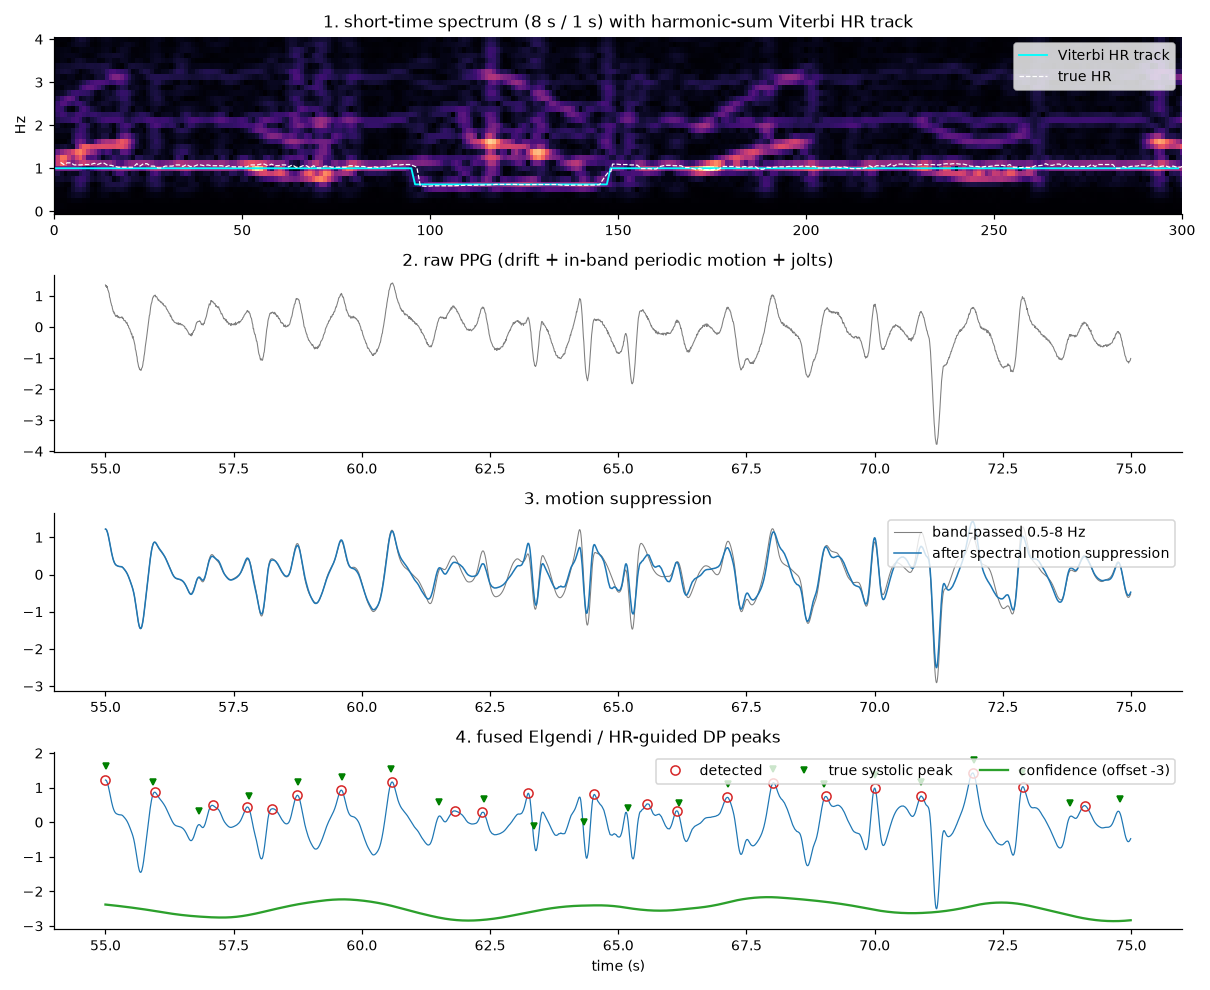
\includegraphics[height=0.78\textheight,keepaspectratio]{fig2_ppg_motion.png}
\column{0.36\textwidth}
\small
\begin{enumerate}
  \item Spectrogram with the Viterbi heart-rate track (cyan) against the true heart rate.
  \item Raw PPG: drift, in-band motion and jolts.
  \item Before and after spectral motion removal.
  \item Fused beat detections and the confidence score.
\end{enumerate}
\vspace{2mm}
\scriptsize\color{gray} Synthetic test signal, motion level 0.5.
\end{columns}
\end{frame}

\begin{frame}
\frametitle{Step 5: Beat Detection with Two Detectors}
\begin{columns}[T]
\column{0.49\textwidth}
\begin{block}{A. Threshold detector}
\footnotesize
\begin{itemize}
  \item \textbf{ECG, Pan--Tompkins:} 5--15\,Hz band $\to$ derivative $\to$ square $\to$ 150\,ms moving average
        $\to$ adaptive threshold; 250\,ms refractory \plain{no two beats closer}; search-back for missed beats.
  \item \textbf{PPG, Elgendi:} 111\,ms and 667\,ms moving averages, local 10\,s offset, 300\,ms refractory.
\end{itemize}
\end{block}
\begin{block}{B. Heart-rate-guided selector}
\footnotesize
\textbf{Dynamic programming} \plain{picks the best whole sequence at once}: candidate peaks are scored by rise
amplitude; the chosen sequence maximises total score minus a penalty for straying from the expected IBI (weight 3).
Real dropped beats survive (tolerance 0.3).
\end{block}
\column{0.48\textwidth}
\begin{exampleblock}{Noise-gated fusion (per 10\,s window)}
\footnotesize
\begin{enumerate}
  \item $\geq$90\,\% of beats agree within 100\,ms $\Rightarrow$ keep A.
  \item Window is clean (noise ratio $<$ 0.45 ECG, $<$ 0.20 PPG) $\Rightarrow$ keep A, \textbf{even if the rhythm
        is irregular}.
  \item Otherwise keep the steadier sequence, biased towards A (1.25 ECG, 2.2 PPG).
\end{enumerate}
\end{exampleblock}
\begin{alertblock}{Why two?}
\footnotesize B is robust to noise but expects a regular rhythm. Rule 2 stops it erasing real atrial
fibrillation (AF).
\end{alertblock}
\end{columns}
\end{frame}

\begin{frame}
\frametitle{Steps 6--7: Peak Refinement, IBI and Confidence}
\begin{block}{Peak refinement and IBI}
\begin{itemize}
  \item \textbf{Parabolic interpolation} \plain{a tiny parabola through the top 3 samples} gives timing finer than
        one sample.
  \item ECG: detect whether beats point up or down, then snap each peak to its tip.
  \item IBI = time between consecutive peaks; IBIs outside 0.25--3\,s are ignored by the rules.
\end{itemize}
\end{block}
\begin{exampleblock}{Confidence score: ``a real beat looks like its neighbours''}
\begin{itemize}
  \item Per beat: correlation with the median \textbf{template} of beats within 5\,s $\times$ amplitude
        consistency $\times$ validity.
  \item Interpolated to every sample, smoothed over 2\,s.
  \item Forced to 0 in gaps over 3\,s, on clipped or flat samples and in invalid regions.
\end{itemize}
\end{exampleblock}
\end{frame}

\begin{frame}
\frametitle{Step 8: Five Explainable Anomaly Rules}
\small
Reference IBI = median of the previous 8 valid IBIs. Rules run only when both beats have quality $\geq$ 0.5.
\vspace{1mm}
\begin{block}{}
\footnotesize
\begin{tabular}{@{}p{0.27\textwidth}p{0.66\textwidth}@{}}
\toprule
\textbf{Rule} & \textbf{Fires when}\\
\midrule
Pause / dropped beat & IBI $>$ 1.5$\times$ reference, or IBI $>$ 2\,s\\
Bradycardia (slow heart) & 5-beat median heart rate $<$ 45\,bpm\\
Premature beat & IBI $<$ 0.8$\times$ reference and IBI + next $>$ 1.6$\times$ reference\\
Ectopic shape (ECG only) & template correlation $<$ 0.8, neighbours $>$ 0.9, IBI $<$ 0.92$\times$ reference\\
AF-type irregularity & 16-beat window: median $|\Delta$IBI$|$/median IBI $>$ 0.10 \textbf{and} nRMSSD $>$ 0.15
                       \textbf{and} (turning-point test \textbf{or} Poincar\'e SD1/SD2 $>$ 0.6)\\
\bottomrule
\end{tabular}
\end{block}
\begin{itemize}
  \item Flagged spans less than 6\,s apart are merged.
  \item \code{-{}-events} exports each episode with its rule and a plain-text reason.
\end{itemize}
\end{frame}

\begin{frame}
\frametitle{Example: Catching the Heart Block in \code{ecg.csv}}
\begin{columns}[T]
\column{0.6\textwidth}
\centering
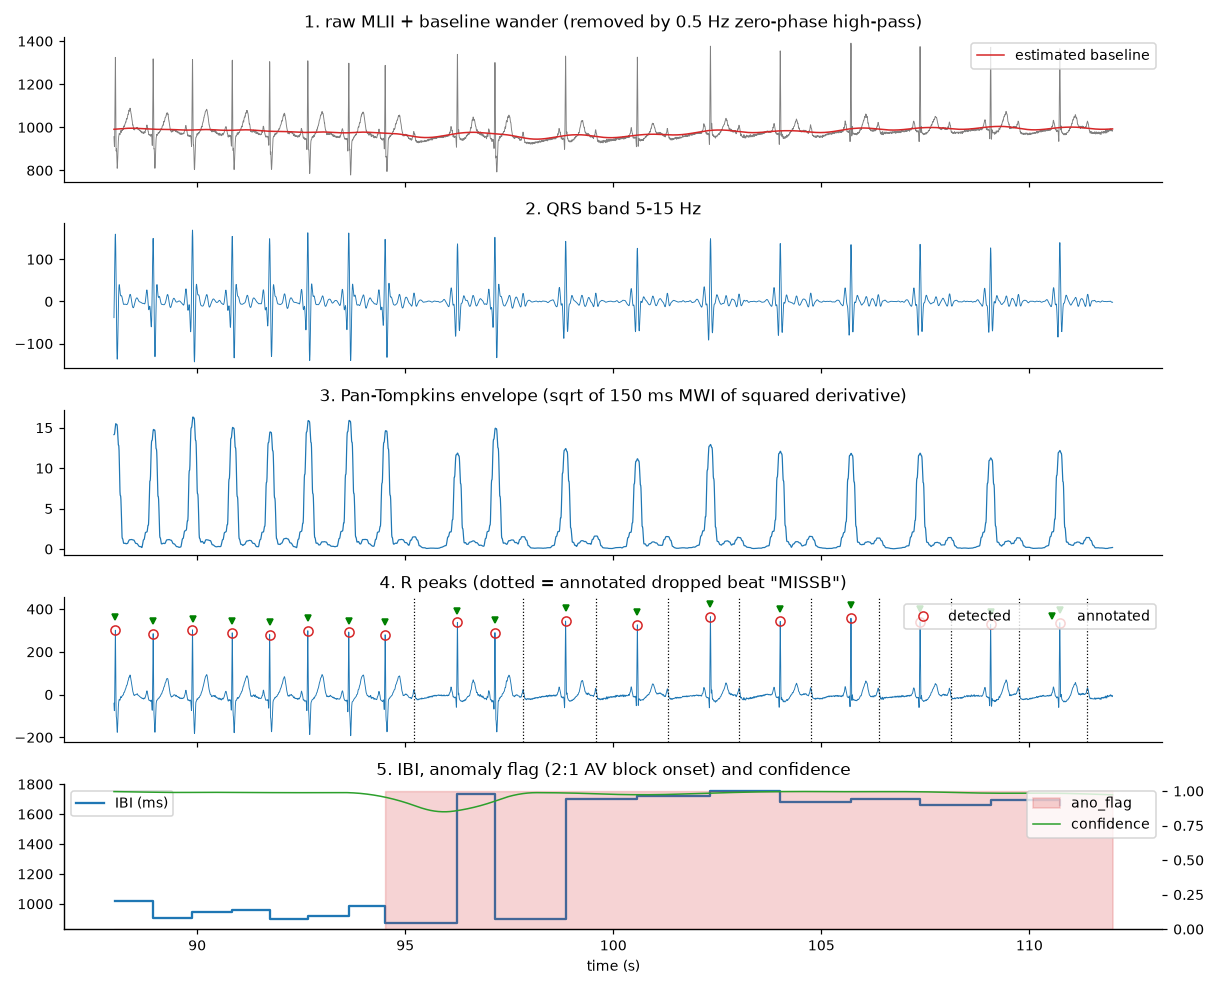
\includegraphics[height=0.8\textheight,keepaspectratio]{fig1_ecg_stages.png}
\column{0.38\textwidth}
\small
\begin{itemize}
  \item Panels: raw signal and drift $\to$ QRS band $\to$ Pan--Tompkins envelope $\to$ detected vs annotated peaks
        $\to$ IBI, flag and confidence.
  \item At onset the IBI jumps from about 960 to 1660\,ms, which is $>$ 1.5$\times$ the reference, so the
        \textbf{pause} rule fires.
  \item During the block the heart rate is about 36\,bpm ($<$ 45), so the \textbf{bradycardia} rule keeps it
        flagged.
\end{itemize}
\end{columns}
\end{frame}

%----------------------------------------------------------------------------------------
\section{Testing and Results}
%----------------------------------------------------------------------------------------
\begin{frame}
\frametitle{How We Tested}
\begin{columns}[T]
\column{0.55\textwidth}
\begin{block}{Test data with known answers}
\small
\begin{itemize}
  \item \code{ecg.csv} (record 231) with annotations.
  \item Record 231 + real NSTDB noise: electrode motion, muscle, baseline wander at 12 / 6 / 0\,dB.
  \item Seven real MIT-BIH arrhythmia records.
  \item \textbf{Synthetic} PPG from real beat times: pulse about 220\,ms after each beat, breathing, drift,
        in-band motion bursts and jolts.
  \item Two independent synthetic PPG fixtures, with and without an accelerometer.
\end{itemize}
\end{block}
\column{0.42\textwidth}
\begin{exampleblock}{Metrics}
\small
\begin{itemize}
  \item A beat counts if within $\pm$150\,ms of a true beat.
  \item Sensitivity \plain{true beats found}, precision \plain{detections that are real}, F1 \plain{their balance}.
  \item IBI mean absolute error (MAE).
  \item Anomaly F1, per sample.
\end{itemize}
\end{exampleblock}
\end{columns}
\end{frame}

\begin{frame}
\frametitle{Results}
\begin{block}{}
\small
\begin{tabular}{@{}lccc@{}}
\toprule
\textbf{Data source} & \textbf{Beat F1} & \textbf{IBI MAE} & \textbf{Anomaly F1}\\
\midrule
\code{ecg.csv} (real clean ECG; also used for tuning) & 1.000 & 0.99\,ms & 0.992\\
44 team-built stress sets (incl.\ synthetic PPG), mean & 0.925 & -- & 0.878\\
Synthetic PPG fixture \textbf{with} accelerometer & 0.996 & -- & 0.865\\
Synthetic PPG fixture \textbf{without} accelerometer & 0.943 & -- & 0.730\\
\midrule
Worst: ECG + electrode-motion noise at 0\,dB & 0.776 & -- & 0.484\\
Worst: synthetic PPG with strong motion & 0.72--0.74 & -- & --\\
\bottomrule
\end{tabular}
\end{block}
\begin{itemize}
  \item Runtime: about 2\,s for a 30-minute record (from our report).
  \item The confidence score drops where accuracy drops, so the output says when not to trust it.
\end{itemize}
\end{frame}

\begin{frame}
\frametitle{Design by Measurement}
\framesubtitle{Two full design branches, one scorer}
\begin{columns}[T]
\column{0.64\textwidth}
\centering
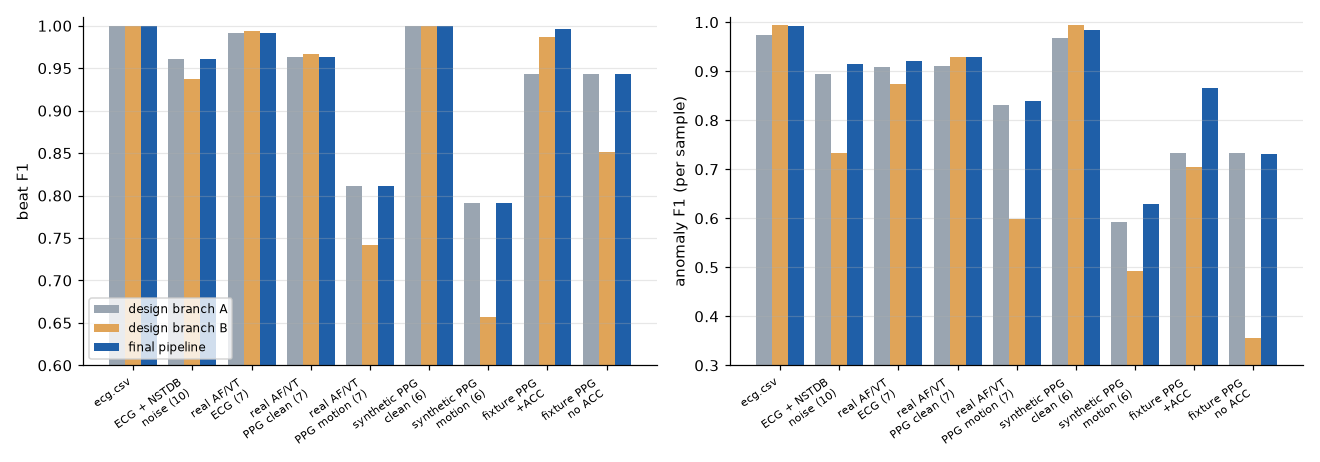
\includegraphics[width=\linewidth,keepaspectratio]{fig5_compare.png}
\column{0.34\textwidth}
\small
\begin{itemize}
  \item We built two complete designs (A and B) and scored them on identical files.
  \item The final pipeline keeps the better component from each.
  \item 44 sets, beat / anomaly F1:
  \begin{itemize}
    \lev A: 0.925 / 0.860
    \lev B: 0.892 / 0.774
    \lev \textbf{Final: 0.925 / 0.878}
  \end{itemize}
\end{itemize}
\end{columns}
\end{frame}

%----------------------------------------------------------------------------------------
\section{Contribution and Limitations}
%----------------------------------------------------------------------------------------
\begin{frame}
\frametitle{What Is New}
\small The building blocks (Butterworth, Pan--Tompkins, Elgendi, NLMS, Viterbi, template quality) are published
methods. Our contribution is how they are combined:
\vspace{2mm}
\begin{exampleblock}{Contributions}
\begin{itemize}
  \item \textbf{Noise-gated fusion} of a threshold detector and a heart-rate-guided selector, so irregular rhythms
        such as AF are not erased.
  \item \textbf{Spectral motion removal} that works without an accelerometer.
  \item \textbf{Design by measurement}: two full branches benchmarked head to head.
  \item \textbf{Explainable output}: every anomaly has a named rule and a reason.
\end{itemize}
\end{exampleblock}
\end{frame}

\begin{frame}
\frametitle{Limitations}
\begin{alertblock}{Current limits}
\begin{itemize}
  \item All PPG test data is synthetic; there is no real-PPG validation yet.
  \item No score on the hidden test set is available to us.
  \item Tuned on our own test sets, so scores may be lower on unseen data.
  \item Very strong in-band motion lowers accuracy.
  \item PPG peaks are not shifted back by the $\sim$250\,ms pulse travel time.
  \item Offline processing; a research prototype, not a diagnostic device.
  \item The AF rule needs 16 beats; very short events fall to the premature-beat and pause rules.
\end{itemize}
\end{alertblock}
\end{frame}

\begin{frame}[fragile]
\frametitle{Demo}
\begin{block}{Generate a test signal (no external data needed) and run}
\scriptsize
\begin{verbatim}
python3 dev/make_fixtures.py --out-dir demo_data
python3 pipeline.py -i demo_data/ppg_acc.csv -o demo_data/pred_acc.csv \
        --annotation demo_data/ppg_acc_ann.txt --events demo_data/events_acc.json
\end{verbatim}
\end{block}
\begin{exampleblock}{What to look at}
\small
\begin{itemize}
  \item The summary line: sampling rate, resampled, accelerometer used, beats, heart rate.
  \item The accuracy line printed against the annotations.
  \item \code{events\_acc.json}: each anomaly episode with its rule and reason.
\end{itemize}
\end{exampleblock}
\end{frame}

\begin{frame}[plain]
\vfill
\centering
{\Huge Thank you}\\[3ex]
{\Large Questions?}\\[4ex]
\small Team Ramanujan: Darshan, Piyush
\vfill
\end{frame}

\end{document}
